%%This is a very basic article template.
%%There is just one section and two subsections.
\documentclass[12pt,  a4paper]{scrartcl}
\usepackage[latin1]{inputenc}
\usepackage[T1]{fontenc}
\usepackage{graphicx}
\usepackage{epstopdf}
\usepackage{avant}
\usepackage[ngerman]{babel}
\usepackage[a4paper, top=3cm, bottom=3cm, left=2.5cm,
right=1.5cm]{geometry}
\usepackage{fancyhdr}
\usepackage{listings}
\usepackage{paralist}
\usepackage{color}
\usepackage{wrapfig}


\definecolor{darkblue}{rgb}{0,0,.5}
\usepackage{hyperref}
\hypersetup{colorlinks=true, breaklinks=true, linkcolor=darkblue,
menucolor=darkblue, urlcolor=darkblue}
\usepackage{breakurl}

\usepackage{url}

\usepackage[cc]{titlepic}
\usepackage{graphicx}
\titlepic{
\includegraphics{images/Xtext-logo-dark.eps}}


\usepackage{tabularx}

\addtokomafont{sectioning}{\color{darkblue}}
\addtokomafont{subsubsection}{\color{darkblue}}

\usepackage{lmodern}


% Setzen des Headers
\setlength{\headwidth}{\textwidth}
\fancyhead[L]{\raisebox{-0.05cm}{
\includegraphics[height=0.6cm]{images/itemis_logo_4c.eps}}}
\fancyhead[R]{\fontfamily{pag}\selectfont{\textbf{LWC13 -
\raisebox{-0.09cm}{
\includegraphics[height=0.5cm]{images/Xtext-logo-dark.eps}} Submission}}}

% Wir wollen eine "Fancy" Ausgabe
\pagestyle{fancy}

% Absatzformatierung
\frenchspacing
\parindent 0pt      % kein Einrcken bei neuem Absatz
\parskip 10pt    	% Abstand zwischen den Absaetzen

% Listingsformatierung
\lstloadlanguages{Java, XML}
\lstset{
    language=Java,
    showspaces=false,
    showstringspaces=false,
    basicstyle=\small\ttfamily\footnotesize,
    columns=fullflexible,% typewriter font look better with fullflex
    keywordstyle=\color[rgb]{0.627,0.165,0.467},
    stringstyle=\color[rgb]{0.286,0.172,0.980},
    commentstyle=\color[rgb]{0.294,0.565,0.478},
    tabsize=2,
    numbers=left,
    numberstyle=\scriptsize,
    breaklines=true,
    identifierstyle=\ttfamily,
    backgroundcolor=\color[rgb]{0.9, 0.9, 0.9},
    rulesepcolor=\color[rgb]{0.3, 0.3, 0.3},
    captionpos=b,
    frame=shadowbox,
    otherkeywords={@SuppressWarnings,@Singleton,@Check,@Inject}
}
\lstdefinelanguage {Xtext}[]{Java} {
    morekeywords={returns,generate,as,import,with,grammar}
}
\lstdefinelanguage {Xtend}[]{Java} {
    morekeywords={def,dispatch,override,val,IF,ENDIF,FOR,ENDFOR,BEFORE,AFTER,SEPARATOR,typeof,@Inject,extension}
%    otherkeywords={+=,=,\{,\}}
}
\lstdefinelanguage {Mwe2}[]{Java} {
    morekeywords={module,var,component,bean}
}
\lstdefinelanguage {dmodel}[]{Java} {
    morekeywords={datatype,entity,op,\:}
}
\lstdefinelanguage {QL}[]{Java} {
    morekeywords={form,\:}
}
\lstdefinelanguage {QLS}[]{Java} {
    morekeywords={page, section, uses, question, font-style, font-color, font-type, widget, navigation, CheckBox, Radio,\:}
}
\lstdefinelanguage {Xbase}[]{Java} {
    morekeywords={val,var,\:}
}
\lstdefinelanguage {instances}[]{Java} {
    morekeywords={\=}
}


%
%%% Trennungsregeln fuer das gesamte Dokument.
%
\hyphenation{language-work-benches domain-model
Generate-Domain-model-Language}

\renewcommand{\baselinestretch}{1.25}

\begin{document}
\begin{titlepage}

\begin{center}

% Upper part of the page
\raisebox{-6cm}{
  
\includegraphics[width=10cm]{./images/Xtext-logo-dark.eps}
}
\\[3cm]


% Title
\rule{\linewidth}{0.7mm}
\\[0.4cm]


    \fontfamily{pag}\selectfont
    \LARGE{\color{darkblue}Language Workbench Challenge 2013 \\
    Xtext Submission} \\[0.5cm]

    \color{black}
    \large{Version: 1.0 - DRAFT \today}
%    \large{Version: 1.1 DRAFT - \today}
    \\[0.4cm]
\rule{\linewidth}{0.7mm}
\\[1.5cm]
\normalfont

% Author
\fontfamily{pag}\selectfont
Karsten Thoms, Johannes Dicks, Thomas Kutz (itemis)
\normalfont

\vfill

% Bottom of the page
%{\large \today}

\end{center}

\end{titlepage}  


\newpage

\section*{Abstract}
The Language Workbench Competition 2011 (LWC11) is an initiative created by a
group of experts at the CodeGeneration 2010
conference\footnote{\url{http://www.codegeneration.net/cg2010/}}. The aim is to
set a common task\footnote{see \url{http://www.languageworkbenches.net/} for the
detailed description of the LWC11 competition and other submissions}
for Language Workbenches\footnote{\url{http://martinfowler.com/articles/languageWorkbench.html},
\url{http://blog.efftinge.de/2007/11/definition-of-term-language-workbench.html}}
which is implemented with the different existing alternatives in a comparable
way. This document describes in detail how the task is solved with
Xtext\footnote{\url{http://www.xtext.org}}. Xtext is one of the most well known
Language Workbenches and part of the Eclipse Modeling
Project\footnote{\url{http://www.eclipse.org/modeling}}.


\section*{Testimonial}
This project was developed with the help of some colleagues at itemis, and I am
grateful for their help:

\begin{compactenum}
  \item \emph{Sven Efftinge} contributed the Instance DSL. Without his knowledge
  it would be very hard to implement this project already with Xtext 2.0 in this
  pre-release state.
  \item \emph{Rainer Klute} has written the initial version of the introduction.
  Although at that time the task was realized with Xtext 1.0.2 and many places
  have been reworked, major parts of the Overview and Phase 0.1 descriptions are
  based on his contribution.
  \item \emph{Karsten Nolte and Alexander Hannweg} initially transformed the
  Wiki pages to LaTeX.
  \item \emph{The Xtext Development Team} was always responsive for questions
  , provided with the Domainmodel example a good template to create major parts
  of the implementation and was eager to fix detected bugs.
  \item Detailed feedback helped to improve the document. My thanks for
  reading the document carefully and providing input go to
  \footnote{Not all from itemis}
  : \emph{Markus V�lter, J�rg Reichert, Joel W. Denton}
\end{compactenum}

\newpage
\section*{Document History}

\textbf {Version 0.1 - 2013-01-28}
\begin{compactitem}
\item Initial creation \\
\end{compactitem}

\textbf {Version 1.0 - 2013-04-08}
\begin{compactitem}
\item Final version for the Language Workbench Challenge workshop in Cambridge
\\
\end{compactitem}


\newpage

\renewcommand{\contentsname}{Table Of Contents}
\setcounter{tocdepth}{4}
\tableofcontents

\newpage

\normalsize

\section{Introduction}

\subsection{Task Description}
The {\href{http://www.languageworkbenches.net/images/5/53/Ql.pdf}{LWC13 task}}
is to implement a DSL for questionnaires (Questionnaire Language, QL), which
basically allows the definition of forms with questions.


\subsection{Technology Stack}
This tutorial expects that you are somehow familiar with Java and Eclipse and
have heard about \url{EMF} and how it works in general before. We start almost at the
beginning, but not quite :-) 

We will use Xtext 2.3.1, which is at the moment of writing the latest official
release.
Xtext 2.4 is in preparation and will be released with Eclipse Kepler in June
2013\footnote{\url{http://wiki.eclipse.org/Kepler/Simultaneous_Release_Plan}}.
The solution approach described here would work also with any version
of Xtext >= 2.0, but the API might differ slightly, so there is no guarantee
that each codeline printed here would work exactly with all versions. For better
reproduction it is highly recommended to use the versions mentioned above.

For Code Generation we will use the language Xtend, which itself is based on
Xtext. Xtend makes use of a common expression language shipped with Xtext called
Xbase. The languages developed here will also be based on Xbase, but more on
this later.

The reference implementation of the Xtend generator will generate, 
JavaServer Faces 2.1( JSF).\footnote{\url{http://www.javaserverfaces.org/}} 
JSF is part of the Java Enterprise Edition (Java EE). It is useful to have a 
basic understanding of how web applications work even if JSF provides a nice level 
of abstraction. The JSF reference implementation from 
Oracle Mojarra 2.1.6\footnote{\url{http://javaserverfaces.java.net/}} is able to run 
within the well known Servlet container Apache Tomcat( v7.0).\footnote{\url{http://tomcat.apache.org/}} 

To get a nicely integrated developement environment we will install some components of the
Web Tools Platform( WTP)\footnote{\url{http://www.eclipse.org/webtools/}} into an existing Eclipse installation.
\subsection{Installing Eclipse and Xtext}

Xtext is a SDK for the \href{http://www.eclipse.org/}{Eclipse} IDE. To
install it you have two options:

\begin{compactitem}
    \item You can download Xtext separately and install it in your Eclipse
    instance.
    \item You can download a specially-crafted complete Eclipse distribution
    which has Xtext prepackaged already.
\end{compactitem}

We will take the latter approach here and describe the individual steps:

\begin{compactenum}
    \item Go to the \href{http://xtext.itemis.com/xtext/language=en/36553/downloads/}{Xtext download
    page}. Here you can get Eclipse 4.2.x (Juno) including Xtext 2.3.1
    along with some tools Xtext depends on. The latter are subsumed here under
    ``Xtext'' for simplicity.
    If you want you can download also a distribution
    which is already bundled with Eclipse 4.3.0 Kepler, but be aware that this
    is not finalized until end of June 2013.
    \item The Eclipse/Xtext distribution is available for multiple platforms.

    \begin{compactenum}
      \item
      \href{http://download.itemis.com/distros/eclipse-SDK-4.2-Xtext-2.3.1-linux-gtk-x86_64.tar.gz}{Linux GTK x86 64 bit}
      \item
      \href{http://download.itemis.com/distros/eclipse-SDK-4.2-Xtext-2.3.1-linux-gtk.tar.gz}{Linux GTK x86 32 bit}
        \item
        \href{http://download.itemis.com/distros/eclipse-SDK-4.2-Xtext-2.3.1-macosx-cocoa-x86_64.tar.gz}{Mac OSX x86 64 bit}
        \item
        \href{http://download.itemis.com/distros/eclipse-SDK-4.2-Xtext-2.3.1-win32-x86_64.zip}{Windows 64 bit}
        \item
        \href{http://download.itemis.com/distros/eclipse-SDK-4.2-Xtext-2.3.1-win32.zip}{Windows 32 bit}
    \end{compactenum}

    \item Unpack the downloaded archive file in a directory of your choice.

        Example (Linux):

\begin{lstlisting}
  cd /opt/local
  gzip -dc /download/eclipse-SDK-4.2-Xtext-2.3.1-linux-gtk-x86_64.tar.gz | tar
  xvfp -
\end{lstlisting}

        The archive will be extracted to a new directory named \texttt{eclipse}. Before
        unpacking the archive, please ensure that there is no subdirectory named
        \texttt{eclipse} yet! Different operating systems may require different unpacking
        methods.\footnote{On Windows do not unpack it into a deep directory,
        since this might cause troubles with long path names.}

    \item Start Eclipse by running the \texttt{eclipse} executable in the newly-created
    \texttt{eclipse} directory.
\end{compactenum}

\subsection{Workspace Setup}

Before we begin, start Eclipse and set up a fresh workspace.

Some settings should be done. Open the workspace settings:

\begin{compactitem}
    \item Windows: Window / Preferences
    \item Mac: Eclipse / Preferences
\end{compactitem}

\paragraph{Workspace Encoding}
$\;$ \\
File encoding is important to some type of files. It is better that the
workspace is set to a common encoding to avoid any platform specific encoding.
By default the workspace is using platform encoding, which is Cp1252 on Windows
and MacRoman on Mac. We will use ISO-8859-1 as a common encoding here.

\begin{compactitem}
    \item Open Eclipse Preferences and go to \emph{General / Workspace}
    \item Change setting \emph{Text file encoding} to \emph{Other /
    ISO-8859-1}
\end{compactitem}

\paragraph{Launch Operation}
$\;$ \\

\begin{compactitem}
    \item Open Run/Debug / Launching
    \item Change ``Launch Operation'' to ``Always
    launch the previously launched application''
\end{compactitem}
This will allow you re-running the previous launched application by just
pressing the Run or Debug button in the Eclipse toolbar, or using keyboard
shortcuts. The default settings does not always do what you want.



\section{Developing the Questionnaire Language}

\section{Developing the Questionnaire Language}

Step 1: Set up initial language implementation
- Create Project
- Define Grammar
- Generate Implementation

\subsection{Generate Language Implementation}

Now that the initial grammar of the language has been defined it is time to test
the language. Xtext ships with a code generator which generates all the glue
code needed for the language implementation.

To generate the code, we need to execute the generator workflow
\texttt{GenerateQlDsl.mwe2}. For this, select the workflow file, open the context menu
and select \emph{Run As / MWE2 Workflow}.

The generator will print some information to the Console, and finally it should
print \texttt{``Done.''}.

\begin{lstlisting}
0    [main] INFO  lipse.emf.mwe.utils.StandaloneSetup  - Registering platform
uri ....
   ...
13727 [main] INFO  .emf.mwe2.runtime.workflow.Workflow  - Done.
\end{lstlisting}

After successful execution the projects will be filled with implementation code.
Code that will be regenerated each time the generator is executed will go to the
source folder \texttt{/src-gen} (in all three projects), whereas code generated to
\texttt{/src} will be generated only once as skeleton. It is safe to edit these
classes.

Xtext follows the Generation Gap
Pattern\footnote{\url{http://heikobehrens.net/2009/04/23/generation-gap-pattern/}}:
Generated code is based on the Xtext API. Manual code is separated from
generated code. Often manual classes are derived from generated classes to allow
overriding of generated code or adding functionality.

Investigate the generated code a bit. Some pieces to mention:
\paragraph{Runtime Project - folder \texttt{src}}
\begin{itemize}
\item The class \texttt{QlDslRuntimeModule} is a Guice configuration.
Guice\footnote{\url{http://code.google.com/p/google-guice/}} is a famous
Dependency Injection\footnote{\url{http://en.wikipedia.org/wiki/Dependency_injection}} framework in Java. 
Xtext makes heavy use of Dependency Injection, which in turn allows to exchange
nearly every bit of the framework for customizing or to work around limitations,
if necessary, without the need to change the framework itself.
\item Class \texttt{QlDslStandaloneSetup} is needed when using the language in
``standalone mode'', i.e. without an Eclipse environment. Eclipse plugins, like
Xtext and the language plugin, usually need an OSGi container as execution
environment. Xtext is designed to be executable without the need to be
deployed into an OSGi container, but for this certain registrations are
required which an OSGi container would usually provide automatically. This is
especially useful when Xtext based languages are used in build environments or
other IDEs.
\item Class \texttt{QlDslFormatter} allows the implementation of a declarative
code formatter for the DSL.
\item File \texttt{QlDslJvmModelInferrer.xtend} is a class implemented with the
Xtend language. The JVM Model Inferrer will play an important role later when we
introduce expressions and code generation.
\item Class QlDslJavaValidation allows the implementation of validation rules
for the DSL.
\end{itemize}


\paragraph{Runtime Project - folder \texttt{src-gen}}
\begin{itemize}
  \item The Ecore metamodel is generated to file \texttt{QlDsl.ecore}.

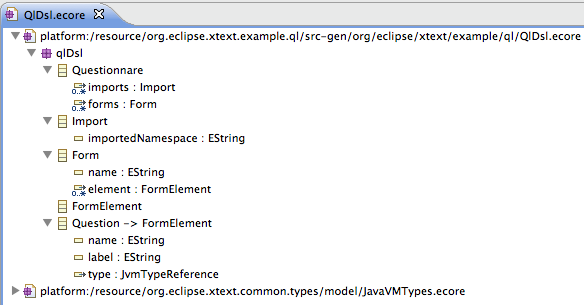
\includegraphics[width=16cm]{./images/chapter01/QlDsl_ecore.png}

  \item The Java implementation code for the metamodel can be found in the
  package \newline\texttt{org.eclipse.xtext.example.ql.qlDsl}.
  \item The package \texttt{org.eclipse.xtext.example.ql.parser.antlr.internal}
  contains an \newline ANTLR3\footnote{\url{http://www.antlr.org}} grammar and
  the Lexer and Parser classes generated from it.
\end{itemize}


\section{Testing the Questionnaire Language}

\subsection{Creating a Launch Configuration}

In order to test the language and the editor we need to deploy the developed
plugins within another Eclipse instance. For testing the easiest way is start a
so-called Runtime Instance.

Open the dialog \emph{Run / Run Configurations} and select the node \emph{Eclipse
Application} from the left tree widget and press the icon with the +
sign to create a new Launch Config.

You could leave the defaults here or change the name and location like in the
screenshot.

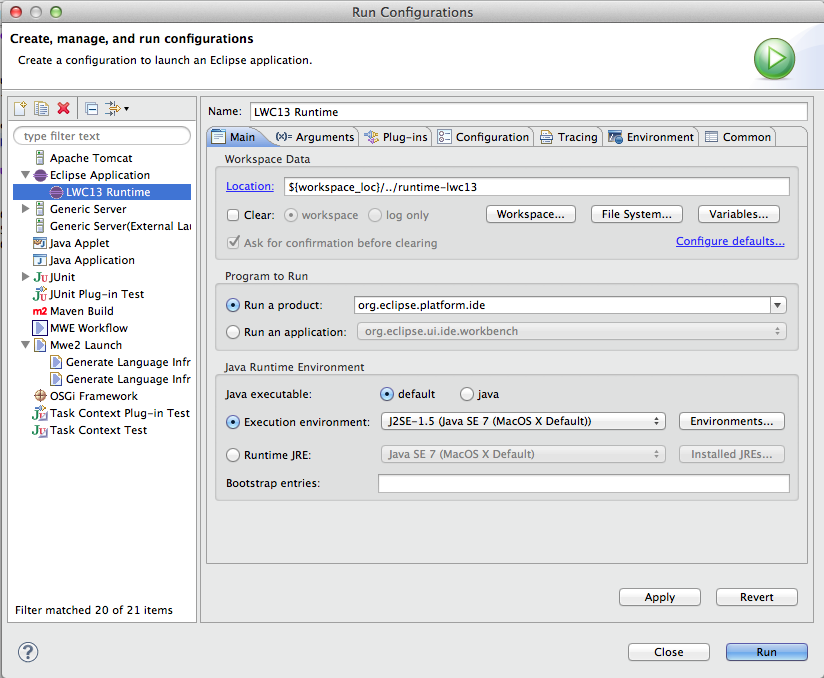
\includegraphics[width=17cm]{./images/chapter01/LaunchConfig.png}

Now switch to the Arguments page and enter in the ``VM arguments'' text box:
\begin{lstlisting}
-Xms40m -Xmx512m -XX:MaxPermSize=150m
\end{lstlisting}
Especially important is the MaxPermSize setting, since the default size of the
PermGen space of the VM (64MB) often is not enough.

Now press the \emph{``Run''} button. Another Eclipse instance will start with an
empty workspace. Close the Welcome window.


\subsection{Create Test Project}

In the Runtime Workspace create a new Java Project with name ``QLTest''.

Select the \texttt{/src} folder and create a new file
\texttt{``housepurchase.ql''}. Once you have created the file a popup dialog
will appear to ask, if you would like to add the Xtext nature on this project.
Answer with ``Yes''.

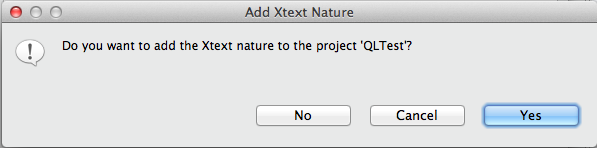
\includegraphics[width=12cm]{./images/chapter01/AddXtextNature.png}

From now on your project will be considered to contain files that Xtext should
recognize (\texttt{.ql} files). Projects having the Xtext nature will be processed by the
Xtext Builder when building projects, other projects are ignored. The Xtext
Builder indexes the Xtext based resources, links the cross-references in the
editor, and validates the model files. On errors, resource markers are created
which can be seen in the editor and the \emph{Problems View}.


\subsection{Xbase}

The language developed in section \ref{sec:DefiningGrammar} does not yet meet all 
demands on the LWC2013 task. Two core features are missing: First, a question's 
answer can be computed, i.e. its answer can be derived from an expression referring 
to previous questions' answers. Second, questions can be optional depending on the 
previous answers. For this, also the possibility to define expressions is needed. This
is where Xbase comes into play.

Xbase is an expression language which can be reused in your own Xtext DSL. Its language
concepts are similar to Java, but with some syntactical derivations improving readability.
The Xbase grammar is defined in Xtext, thus its elements can be used in any other Xtext grammar
by importing or directly extending Xbase via Xtext's possibility for grammar inheritance.
In addition to the grammar, Xbase ships with further infrastructural parts like a compiler, 
interpreter, linker or static analyzer which all can be adapted to your own needs. In
the background, Xbase produces plain Java code which is run on the JVM. Like
other DSLs defined with Xtext, Xbase provides also editor features like syntax highlighting, 
content assistance and navigation via hyperlinks. In the following we will first introduce
some language concepts of Xbase, and afterwards we will describe how to integrate Xbase
into the Questionnaire DSL.

In Xbase everything is an expression which always has a return type which might be \texttt{null} 
for some expressions. Variables are defined with the \texttt{var} keyword, whereas for 
constant values the \texttt{val} keyword is used. Types are derived automatically, so they 
don't need to be defined explicitly:

\begin{lstlisting}[language=Xbase]
var myVariable = 'some modifiable value'
val Integer myConstant = 42  
\end{lstlisting}

Xbase ships with a library extending existing Java types like String or Integer with further 
functionality. So besides the already known String operations from Java like 
\texttt{toUpperCase} or \texttt{toLowerCase}, in Xbase expressions you can also use \texttt{toFirstUpper}
and \texttt{toFirstLower} changing only the first letter's case which might come in handy 
in some situations. Large numbers can be written more readable by using underscores to
separate digits:

\begin{lstlisting}[language=Xbase]
"a day has ".toFirstUpper() + 86_400_000 + " milliseconds."
// results in: A day has 86400000 milliseconds.
\end{lstlisting}

As in Java, Xbase provides \texttt{if-else}-expressions for defining conditions. Since each expression
has a return type, it is valid to use  \texttt{if-else}-blocks similar to the ternary operator in Java:

\begin{lstlisting}[language=Xbase]
var x = if (condition) 42 else 43
\end{lstlisting}

There are further concepts in Xbase which we will not cover here in more detail, since they have
not much relevance for the questionnaire language. So e.g. it is possible to use loops for
iterating over a collection of element; there is a \texttt{switch-case}-expression
with type guards allowing for defining behavior depending on the type of a parameter; and last but
not least, Xbase allows the definition of closures. For more details, please look up the reference
documentation\footnote{\url{http://www.eclipse.org/Xtext/documentation.html#xbaseLanguageRef_Introduction}}
or the Xbase tutorials directly in Eclipse (\emph{File / New / Other.. / Xbase Tutorial}). 

With these capabilities integrated in the Questionnaire language it is feasible to define complex
domain logic e.g. for the result of a questionnaire directly in its definition. For example, when
designing a questionnaire for a test, let's say to define a person's stress level, you can write
some Xbase code as expression for the last ``result'' question:

\begin{lstlisting}[language=Xbase]
stressLevelResult: "Your Stress-Level: " String (
	{
		var Integer stressPoints = if (hasTimePressureAtWork) 30 else 0
		stressPoints = stressPoints + daysSleepingBadPerWeek * 3
		stressPoints = stressPoints + glassesOfAlcoholPerDay * 12
		stressPoints = stressPoints - daysWithSportPerWeek * 2
		if (stressPoints>80) "High" else if (stressPoints>40) "Medium" else "Low"
	}
) 
\end{lstlisting}

\section{Including Expressions into the QL Language}

- Derive Grammar from Xbase
- Generate Implementation

\subsection{JVM Model Inference}

For languages using Xbase it is necessary to tell Xtext, how to map concepts of a language to a Java model. In our example,
a Form could be mapped to the Type concept, while Questions are the fields of a class. By doing this, elements of the language
can be made available in expressions. Further, it allows that model elements are linkable where Java types are expected, without
necessarily generate a Java class.

The derivation of the Java model for language concepts is the responsibility of the JVM Model Inferrer, which is a class that implements
the \href{http://download.eclipse.org/modeling/tmf/xtext/javadoc/2.3/org/eclipse/xtext/xbase/jvmmodel/IJvmModelInferrer.html}{\texttt{IJvmModelInferrer}} interface.
A skeleton has already been generated into package \texttt{org.eclipse.xtext.example.ql.jvmmodel}. The file \texttt{QlDslJvmModelInferrer.xtend} is a class
written with Xtend.

The mapping that has to be implemented for the Questionnaire DSL should be as follows:
\begin{enumerate}
  \item Each \texttt{Form} instance is mapped to a \texttt{JvmDeclaredType} (which is the common concept for Java classes and interfaces).
  The type's name is simply the form name, and the target package is forms.
  \item Each \texttt{Question} of a \texttt{Form} is mapped to a \texttt{JvmField}, which is added as member of the declared type
  \item For each \texttt{Question} accessor methods for the field are generated. The field gets only a setter if the value of the Question is
  not computed by an expression. If the field is computed, the content of the getter has to compute the result.
  \item For each \texttt{Question} a method \texttt{is<QUESTIONNAME>Enabled()} is inferred.
  Questions with computed values are not enabled.
  \item For each \texttt{ConditionalQuestionGroup} a method is produced that computes
  whether the group is visible or not. 
\end{enumerate}

Now place the content into the inferrer class\footnote{\url{https://gist.github.com/kthoms/5132153}}
: 
\begin{lstlisting}[language=Xtend]
package org.eclipse.xtext.example.ql.jvmmodel

import com.google.inject.Inject
import java.io.Serializable
import org.eclipse.xtext.common.types.JvmOperation
import org.eclipse.xtext.common.types.util.TypeReferences
import org.eclipse.xtext.example.ql.qlDsl.ConditionalQuestionGroup
import org.eclipse.xtext.example.ql.qlDsl.Question
import org.eclipse.xtext.example.ql.qlDsl.Questionnaire
import org.eclipse.xtext.xbase.XExpression
import org.eclipse.xtext.xbase.XbaseFactory
import org.eclipse.xtext.xbase.jvmmodel.AbstractModelInferrer
import org.eclipse.xtext.xbase.jvmmodel.IJvmDeclaredTypeAcceptor
import org.eclipse.xtext.xbase.jvmmodel.JvmTypesBuilder

class QlDslJvmModelInferrer extends AbstractModelInferrer {
  @Inject extension JvmTypesBuilder
  @Inject TypeReferences typeReferences

def dispatch void infer(Questionnaire element, IJvmDeclaredTypeAcceptor acceptor, boolean isPreIndexingPhase) {
    for (form: element.forms) {
      acceptor.accept(form.toClass("forms."+form.name))
      .initializeLater[
        //implements Serializable
        it.superTypes +=typeReferences.getTypeForName(typeof(Serializable),element,null)

        members += toField("serialVersionUID",typeReferences.getTypeForName("long",element),[final = true ^static = true 
          setInitializer([it.append("1L")])
        ])

        val allQuestions = form.eAllContents.filter(typeof(Question)).toList
        
        for (question: allQuestions) {
          members += question.toField(question.name, question.type)
        }

        for (question: allQuestions) {
          if (question.expression == null) {
            members += question.toGetter(question.name, question.type)
            members += question.toSetter(question.name, question.type)
          } else {
            val getter = question.toGetter(question.name, question.type)
            getter.body = question.expression
            members += getter
          }
          members += question.createIsEnabledMethod
        }

        val allQuestionGroups = form.eAllContents.filter(typeof(ConditionalQuestionGroup)).toList
        var groupIndex=0;
        for (questionGroup: allQuestionGroups) {
          members += questionGroup.createIsGroupVisibleMethod(groupIndex)
          groupIndex = groupIndex+1
        }

      ]
    }
  }

   def JvmOperation createIsEnabledMethod (Question question) {
     question.toMethod("is"+question.name.toFirstUpper+"Enabled", typeReferences.getTypeForName("boolean", question, null)) [
       body = [it.append('''return «question.expression == null»;''')]
    ]
   }

   /** Create a method <code>public boolean isGroup[groupIndex]Visible ()</code>.*/
   def JvmOperation createIsGroupVisibleMethod (ConditionalQuestionGroup group, int groupIndex) {
     group.toMethod("isGroup"+groupIndex+"Visible", typeReferences.getTypeForName("boolean", group, null)) [
       if(group.condition != null) {
         body = group.condition
       } else {
         body = [it.append('''return true;''')]
       }
     ]
   }

}
\end{lstlisting}

Now lets take a deeper look at the implementation:

\begin{lstlisting}[language=Xtend]
class QlDslJvmModelInferrer extends AbstractModelInferrer {
  @Inject extension JvmTypesBuilder
  @Inject TypeReferences typeReferences
  def dispatch void infer(Questionnaire element, IJvmDeclaredTypeAcceptor acceptor, boolean isPreIndexingPhase) {
     ...
  }
}
\end{lstlisting}

The inferrer class implements \texttt{IJvmModelInferrer}, but for convenience we derive
from its abstract implementation \texttt{AbstractModelInferrer}. The main method to
implement is \texttt{infer()}. In the case of QL models, the root element
of model resources is a \texttt{Questionnaire}. The base implementation uses polymorphic dispatching on
the root element of a model resource, and the \texttt{infer()} method of our
implementation hooks into the dispatching by using the dispatch keyword. That is
also why the first argument can be of type \texttt{Questionnaire}, and not of the base
type \texttt{EObject}, like defined in the \texttt{infer()} method that is definied in
\texttt{IJvmModelInferrer}.

The implementation uses two services, which are injected as members into the
class:
\begin{itemize}
\item The \texttt{JvmTypesBuilder} offers factory and builder functions to create
instances of JVM Model types. The additional keyword \texttt{extension} has the effect,
that the methods of the \texttt{JvmTypesBuilder} become so-called \textbf{extension methods}.
This means, the functions become implicitly available as additional
methods on the first argument of the function. We will see extensive use of this
nice feature of Xtend in the implementation of the Xtend based code generator in
the next chapter.
\item \texttt{TypeReferences} is used to retrieve the respective JVM Model instances for
given qualified Java class names through its \texttt{getTypeForName()} methods. 
\end{itemize}

\begin{lstlisting}[language=Xtend]
    for (form: element.forms) {
      acceptor.accept(form.toClass("forms."+form.name))
      .initializeLater[
         ...
      ]
    }
\end{lstlisting}

Let's take a deeper look on the \texttt{infer()} method. The outer loop simply
iterates over the \texttt{Form} instances of the \texttt{Questionnaire} element.
Inside the loop we first derive a Class instance for each \texttt{Questionnaire}
element in package \texttt{forms}. JVM Model Inference is executed in two
phases: In the first phase all types are derived, without any content. In the
second phase, the content of the types is derived. This is done by the closure
passed to \texttt{initializeLater()}. The reason why this has to happen this way
is that during inference of type members, they could refer again to types that
are derived by the inferrer. The two phases prevent circular calls.

\begin{lstlisting}[language=Xtend]
it.superTypes +=typeReferences.getTypeForName(typeof(Serializable),element,null)

members += toField("serialVersionUID",typeReferences.getTypeForName("long",element),
[final = true ^static = true 
  setInitializer([it.append("1L")])
])
\end{lstlisting}
        
We want to make the resulting Java class serializable. This is optional, but
better style. Therefore the class has to implement the \texttt{java.io.Serializable}
interface, whose JVM Model representative is retrieved from the \texttt{TypeReferences}
instance and added to the \texttt{superTypes} collection. The identifier \texttt{it} denotes the
implicit variable of type Form of the closure. It is not necessary to qualify it
here, it could be left out. The closure passed to the \texttt{setInitializer()}
method initializes the field with the value ``1'' of type long.

\begin{lstlisting}[language=Xtend]
val allQuestions = form.eAllContents.filter(typeof(Question)).toList

for (question: allQuestions) {
  members += question.toField(question.name, question.type)
}
\end{lstlisting}

All \texttt{Question} instances from the resource are bound to the final variable
\texttt{allQuestions}. Since Questions can be nested into groups, the content has to be
searched recursively. \texttt{eAllContents} will traverse over all elements.

Next, for each \texttt{Question} a \texttt{JvmField} instance is inferred. Here the
\texttt{JvmTypesBuilder} is helping us with the method \texttt{toField}, which gets the name and
type of the derived field. Here we see the effect of the extension keyword: It
seems that \texttt{toField} is actually a method of type Question, but it is a method of
the \texttt{JvmTypesBuilder} class.

\begin{lstlisting}[language=Xtend]
for (question: allQuestions) {
  if (question.expression == null) {
    members += question.toGetter(question.name, question.type)
    members += question.toSetter(question.name, question.type)
  } else {
    val getter = question.toGetter(question.name, question.type)
    getter.body = question.expression
    members += getter
  }
  ...
}
\end{lstlisting}

The next loop creates the accessor methods for the fields. We could have done
this in the previous loop also, but it is better style to declare the fields
first, and methods next in the class. The inferred \texttt{JvmDeclaredType} will be
translated to Java later, so it is better to have that clean from the beginning.

Within the loop, we decide if the question has a computation expression or not.
If it hasn't one, it is a simple field with getter and setter, where we call the
\texttt{toGetter()}/\texttt{toSetter()} builder functions. If the question value is computed by an
expression, it does not make sense to offer a setter method. The field needs to
be read-only. The getter method does not simply return the value of a field.
Instead, the method has to evaluate the expression. Thus, we assign the
expression as body of the method.

\begin{lstlisting}[language=Xtend]
for (question: allQuestions) {
  ...
  members += question.createIsEnabledMethod
}

...
def JvmOperation createIsEnabledMethod (Question question) {
  question.toMethod("is"+question.name.toFirstUpper+"Enabled",
 typeReferences.getTypeForName("boolean", question, null)) [ body = [it.append('''return «question.expression == null»;''')]
  ]
}
\end{lstlisting}

For each \texttt{Question} a method \texttt{boolean is<QUESTIONNAME>Enabled()}
is inferred. The body of the method does simply return \texttt{true} if the Question does
not have an computation expression assigned, or \texttt{false} otherwise.

In this case we assign to the body a closure that computes the method
implementation text. This is the first example where we make use of Xtend's \emph{Rich
String} feature (the text between the three single quotes '''), which is
later heavily used in the code generator templates.

\begin{lstlisting}[language=Xtend]
val allQuestionGroups = form.eAllContents.filter(typeof(ConditionalQuestionGroup)).toList
var groupIndex=0;
for (questionGroup: allQuestionGroups) {
  members += questionGroup.createIsGroupVisibleMethod(groupIndex)
  groupIndex = groupIndex+1
}

def JvmOperation createIsGroupVisibleMethod (ConditionalQuestionGroup group, int groupIndex) {
 group.toMethod("isGroup"+groupIndex+"Visible", typeReferences.getTypeForName("boolean", group, null)) [
   if(group.condition != null) {
     body = group.condition
   } else {
     body = [it.append('''return true;''')]
   }
 ]
}
\end{lstlisting}

We now filter all \texttt{ConditionalQuestionGroup} instances from the \texttt{Questionnaire} and
loop over them. For each of them, a method \texttt{is<QUESTIONGROUPINDEX>Visible()} 
is produced. Unfortunately, question groups are anonymous, thus we
maintain an index counter and name the methods \texttt{isGroup<IDX>Visible()}.

Since condition expressions for groups are optional, the method body has to
return simply \texttt{true} in the case that no expression is assigned. When groups have
a condition, the condition expression is assigned as the method body.




\section{Developing the Code Generator}

\subsection{Reference Implementation}

Before implementing a code generator one has to know what the target code is. Therefore a reference implementation has been
developed which was coded to large degree manually. From this reference code the templates can be derived. Also this is a
manual step.

We use a Java Server Faces (JSF) based application, which can be deployed on any
Java Web container (also known as a Servlet container) like Glassfish, JBoss and Apache Tomcat.

The following screenshot shows the structure of the web application project. The application is available for download from the project 
homepage (\href{http://lwc13-xtext.eclipselabs.org.codespot.com/files/JSF-QL-1.0.zip}{JSF-QL-1.0.zip})

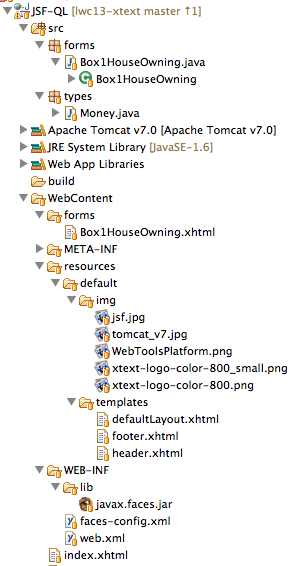
\includegraphics[width=10cm]{./images/chapter02/referenceimpl_projecttree.png}

Large parts of the application are not derivable from the model, they build the skeleton of the project. This is:
\begin{itemize}
\item Custom types (\texttt{src/types/*})
\item Custom type converter (\texttt{src/converter/*})
\item Images (\texttt{WebContent/resources/default/img/*})
\item Page Templates (\texttt{WebContent/resources/default/templates/*})
\item Libraries (\texttt{WebContent/WEB-INF/lib/*})
\item Web Application Descriptor (\texttt{WebContent/WEB-INF/web.xml})
\item Faces configuration (\texttt{WebContent/WEB-INF/faces-config.xml})
\end{itemize}

We will focus on the parts which are dependent on the QL model and thus subject of code generation. These artifacts are:
\begin{itemize}
\item Java Bean classes representing the state of a Form (\texttt{src/forms})
\item JSF enabled XHTML pages representing the presentation of a Form (\texttt{WebContent/forms/*})
\end{itemize}

... to be continued


To integrate the generated artifacts into our web application we have to
make manually changes in the \texttt{welcome-file} declared in \texttt{WebContent/WEB-INF/web.xml} later.
(\texttt{WebContent/index.xhtml})



\subsection{Xtend}
 
Since we will use Xtend to write the code generator, this chapter describes some
basic concepts of the Xtend language. However, we will not cover all aspects of
Xtend in this section, for more information see also the official documentation\footnote{\url{http://www.eclipse.org/xtend/documentation.html}}.

Xtend is a statically-typed general purpose language similar to Java. Xtend uses
Xbase as core language which was already roughly explained in section \ref{sec:Xbase}.
Hence, the presented concepts of Xbase are also valid for Xtend. The main focus
of Xtend lies in providing a language that is more readable than Java in certain
situations. In the backgroud, Xtend compiles to Java code. Thus, it plays perfectly
together with Java, e.g. methods declared in Java classes can be called in Xtend
and vice versa. Several concepts of Xtend are especially beneficial when writing code
generators. 

\begin{lstlisting}[language=Xtend]
def someMethod() {
  var myQuestion = 'where do we go?'
  myQuestion = myQuestion.toFirstLower
  val myAnswer = 42
  'The answer for question '+myQuestion+' is: '+myAnswer
}
\end{lstlisting}

In Xtend, a method is defined with the \texttt{def} keyword. The return type is
optional and will be automatically inferred. Only when a method is recursively
invoking itself, a return type needs to be specified explicitly. The keyword 
\texttt{var} defines a variable; constant values are defined with \texttt{val}.
In Xtend - since it is based on Xbase - everything is an expression, meaning that 
it has a return type. The last expression of a method defines the return value
and also the return type of the method.

In line 3 a so-called extension method is used. Recall that the String class in 
Java does not provide a method \texttt{toFirstUpper}. Xtend allows for extending
closed types without changing (maybe you already guess where Xtend got its name from).
You can easily write your own extension for the String type for example:

\begin{lstlisting}[language=Xtend]
  def square(Integer input) {
  	input * input
  }
  
  def useExtension() {
  	16.square // returns 256
  }
\end{lstlisting}

What Xtend basically does is changing the syntax of how methods are called. Instead
of writing \texttt{toLastUpper(``Hello'')}, Xtend always offers the alternative to
use the first input parameter as receiver of the method call (\texttt{``Hello''.toLastUpper}).
This results in the syntax being more chained than nested which improves readability.
To use methods from another class as extension methods in your class, the field
defining an object of the other class needs to be marked with the \texttt{extension}
keyword. In our scenario we will use dependency injection like the following:

\begin{lstlisting}[language=Xtend]
class MyGenerator implements IGenerator{
  @Inject extension IJvmModelAssociations
  ...
}
\end{lstlisting}

This statement simply allows to use the methods declared by the interface \texttt{IJvmModelAssociations}
in our generator class as extension methods on our objects. Which concrete implementation of the
interface is later actually called, is configured in the Guice module.

A further useful feature of Xtend is \emph{polymorphic dispatching}. Using the \texttt{dispatch}
keyword on multiple methods with identical signatures has the effect that the 
decision on which method should be called is based on the runtime type of the
target object. In contrast, Java binds methods at compile time based on the static
type of the target object. Since Xtend compiles to Java, polymorphic dispatching
is internally realized by a dispatcher method using a cascade of
\texttt{instanceof} constructs. 

\begin{lstlisting}[language=Xtend]
  def dispatch doSomething(Integer input) {
  	// do something with integer
  }
  
  def dispatch doSomething(Float input) {
  	// do something with float
  }
  
  def useDispatching() {
    val Number x = 123
    val Number y = 0.1
    x.doSomething + y.doSomething
  }
\end{lstlisting}

// TODO gescheites beispiel überlegen und zwei sätze zu schreiben.

Xtend offers the possibility to define \emph{rich Strings} (also called \emph{templates})
which is especially useful when writing code generators. Rich Strings allow for
writing complex Strings with line breaks and indentations without the need for
concatenating special characters like \texttt{'\textbackslash n'} or \texttt{'\textbackslash t'}. A rich String
construct starts and ends with triple single quotes (\texttt{'''}). Within such
a String code pieces which themself return a String can be inserted (surrounded by guillemots \texttt{«»}).
There are also logical structures like \texttt{for} loops or \texttt{if-else}
statements supported:

\begin{lstlisting}[language=Xtend]
  def htmlContent(List<String> contents) '''
  	<html>
  	  <body>
  	    «FOR content: contents BEFORE '<p>' SEPARATOR '<br/>' AFTER '</p>'»
  	      «IF content.length > 10»
  	        Large Content: «content.toFirstUpper»
  	      «ELSE»
  	        Small Content: «content.toFirstUpper»
  	      «ENDIF»
  	    «ENDFOR»
  	  </body>
  	</html>'''
\end{lstlisting}

Note the special keywords in the \texttt{FOR} loop declaration: \texttt{BEFORE} 
and \texttt{AFTER} will be called once before and after the iteration, but only
if the loop will be iterated at least once. With the \texttt{SEPARATOR} keyword
a string which will be inserted between two iteratins can be specified. Calling 
the example method with ['hello', 'Some more text'] results in:

\begin{lstlisting}[language=Xtend]
<html>
  <body>
    <p>
    Small Content: Hello<br/>
    Large Content: Some more text
    </p>
  </body>
</html>
\end{lstlisting}

Last but not least, Xtend offers a more sophisticated \texttt{switch-case} statement
than Java does. The \texttt{break} statement as known from Java is implicit in Xtend.
Furthermore, switching based on Strings and even types is possible:

\begin{lstlisting}[language=Xtend]
  def getTypeName(Number input) {
  	switch (input) {
  		Integer: "It is an Integer!"
  		Float:   "It is a Float!"
  		default: "It is some other number type."
  	}
  }
\end{lstlisting}

Now as you know the basic concepts of Xtend, let's finally start writing the code
generator.

\subsection{Code Generator}

In this section you will learn how to implement the code generator for 
the target application. For simplicity, the code generator templates are placed
in the \texttt{org.eclipse.xtext.example.ql} project in a sub-package \texttt{generator}. 
Usually it would be better to create a separate project which contains the generator,
since the language is independent from a single target platform. It would
be possible to create different code generators for different target platforms,
and it would be better to implement each of them as separate projects.

Generator templates in Xtend are implementations of the \texttt{IGenerator}
interface:

\begin{lstlisting}[language=Java]
package org.eclipse.xtext.generator;

public interface IGenerator {
	/**
	 * @param input - the input for which to generate resources
	 * @param fsa - file system access to be used to generate files
	 */
	public void doGenerate(Resource input, IFileSystemAccess fsa);
}
\end{lstlisting}

\subsubsection {Dispatcher template}

The code generator is invoked with a \texttt{Resource} instance, which holds a \texttt{Questionnaire}
instance. We have to generate multiple artifacts for each resource, so it is a common 
pattern to create a template class which serves as entry point and dispatches to other
template classes to create the artifacts. Usually one template per artifact is
created.

Create the class \texttt{Root.java} in package \texttt{org.eclipse.xtext.example.ql.generator}:

\begin{lstlisting}[language=Java]
package org.eclipse.xtext.example.ql.generator;

import javax.inject.Inject;

import org.eclipse.emf.ecore.resource.Resource;
import org.eclipse.xtext.generator.IFileSystemAccess;
import org.eclipse.xtext.generator.IGenerator;
import org.eclipse.xtext.xbase.compiler.JvmModelGenerator;

@SuppressWarnings("restriction")
public class Root implements IGenerator {
  @Inject
  JvmModelGenerator jvmModelGenerator;

  public void doGenerate(Resource input, IFileSystemAccess fsa) {
    // dispatch to other generators
    jvmModelGenerator.doGenerate(input, fsa);
  }
}
\end{lstlisting}

As a first generator to which is dispatched, we inject an instance of
\texttt{JvmModelGenerator}. This is a standard generator shipped with Xtext which
translates types inferred by the Jvm Model Inferrer to Java classes.
In our case, the Java class for Forms are generated by the
\texttt{JvmModelGenerator}. In JSF terms, we speek of the \emph{Backing Bean}.
 
Next, Xtext has to know that \texttt{Root} is the template that has to be invoked
as generator implementation. This has to be configured - you guessed right! - 
with Guice again. We need to add a configuration that binds the \texttt{IGenerator}
interface to the \texttt{Root} class.

Open class \texttt{QlDslRuntimeModule} and add this method:

\begin{lstlisting}[language=Java]
  @Override
  public Class<? extends IGenerator> bindIGenerator() {
    return Root.class;
  }
\end{lstlisting}

Now we are ready to add additional templates and register them in the
\texttt{Root} class.

\subsubsection {JSF Generator}

For that purpose we use the \texttt{New Xtend Class Wizard} to create a
new Xtend file \texttt{JSFGenerator.xtend} in package
\texttt{org.eclipse.xtext.example.ql.generator}.

\begin{center}
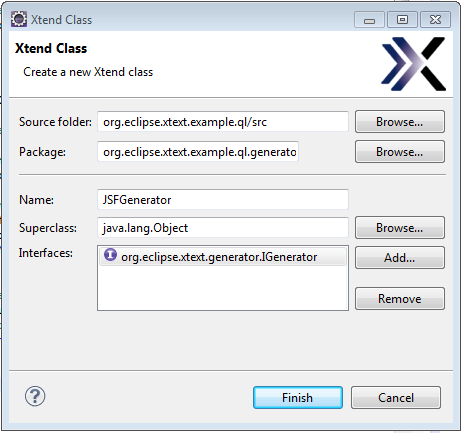
\includegraphics[width=10cm]{./images/chapter02/newXtendClassWizard.png}
\end{center}

The \texttt{New Xtend Class Wizard} provides the possibility to add interfaces
by use of the \texttt{Add} button near the interface section. As we want to
create a new generator we add the interface
\texttt{org.eclipse.xtext.generator.IGenerator} to our new Xtend class.

\begin{center}
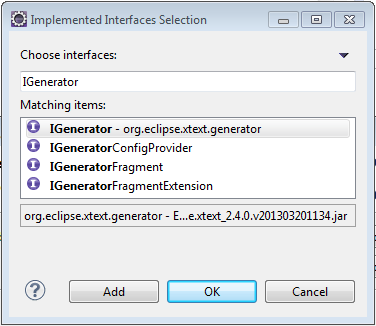
\includegraphics[width=10cm]{./images/chapter02/newXtendClassWizardAddInterface.png}
\end{center}



- create xtend file
- add xtend lib if required
- show whole generater
- explain step by step


\subsection{Testing the Questionnaire Application}
\label{sec:TestingQLApplication}

It's time to test the application we have developed so far. If your runtime
environment is still open you need to restart it. Just switch to the runtime
instance and press \emph{File / Restart}. See also section \ref{sec:TestingQL}
for more information on how to start your runtime evironment for testing. Once
the runtime environement is running you can test the code generator in the
QLText project created in section \ref{sec:TestingQL}. Code generation process
is triggered automatically on the fly when the QL model gets modified. The
generated artifacts are located in folder \texttt{WebContent/generated/forms}.
Into this folder also an \texttt{index.xhtml} file is placed which you can use
as starting point for the questionnaire application. Right-click on the index
file and press \emph{Run As / Run On Server}. In the next dialog choose the
Tomcat server which you should have configured in section
\ref{sec:IDEConfiguration} (if not, then now is the time to do it) and press
\emph{Next}. If your test project is not already in the \emph{Configured} area
then it needs to be moved there by using the \emph{Add >} button. Finally press
\emph{Finish} to start the application in the integrated browser within eclipse.
You can also copy the link and paste it in a web browser of your choice. The
result should be similar to the one on the next screenshot:

\begin{center}
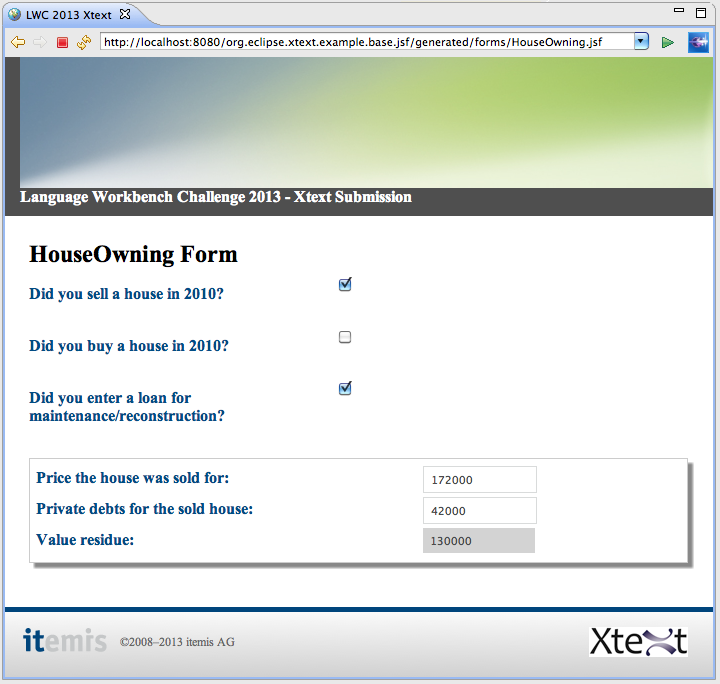
\includegraphics[width=15cm]{./images/chapter02/questionnaireApplication.png}
\end{center}
 
Now it's show time. You can modify your QL model and save it. The XHTML files
will be regenerated on the fly. The server needs some seconds to reload the
backing beans. Afterwards you can press the \emph{Refresh} button and see the
result immediately.



\newpage
\section{Layout and Styling Language (QLS)}

\subsection{The Language QLS}

In this chapter we will describe how the optional task to define a language 
for styling and layout information can be accomplished in our language workbench.
The language QLS should allow for defining the following information:
\begin{itemize}
  \item Grouping of question forms into pages, sections and subsections
  \item Navigation links between pages
  \item Styling of question texts by defining font style, font weight, font
  family and color
  \item Defining the appearance of a question by specifying the widget type to render
\end{itemize}

The following shows an example model that we want to be able to define with QLS:

\begin{lstlisting}[language=QLS]
page HouseOwningPage {
	section house uses Box1HouseOwning {
		question hasBoughtHouse [font-style: "italic"]
		question valueResidue [
			font-weight: "bold" 
			font-color:  "#2233FF"
			font-family: "Arial"
		]
	}
	section garage uses GarageOwning {
		question hasBoughtGarage [widget: Radio["Yepp", "Nope"]]		
	}
	navigation {
		CarOwningPage
	}
}

page CarOwningPage uses CarOwning {
	// ...
}
\end{lstlisting}

This example model defines two pages. The first page consists of two sections,
one for the question form \texttt{Box1HouseOwning} which was defined in chapter 
\ref{chp:QL} and one for a further form called \texttt{GarageOwning}. The form to
be rendered inside a page or a section is specified by the \texttt{uses} keyword.
This definition must be unambiguously, e.g. if there is a form included by a page,
it is not allowed to refer to another form in one of its containing sections.
This restriction is ensured by implementing a corresponding validation. How this
can be done is covered in section \ref{sec:validation}. In a section (or page)
the styling information for the questions of the included form can be defined as
in lines 3-9 and 11. The \texttt{navigation} keyword allows to define the order
in which the pages are to be displayed by specifying which page should appear next.

Before we can write the corresponding Xtext grammar, we need to create the DSL 
projects for QLS as we have done for the Questionnaire language. For this, refer
again to chapter \ref{chp:CreateDslProjects} and replace all occurences of 
\texttt{ql} with \texttt{qls}. The project \texttt{org.eclipse.xtext.example.qls}
should then contain the grammar file \texttt{QlsDsl.xtext}. We define the content
of this file as the following:

\begin{lstlisting}[language=Xtext]
grammar org.eclipse.xtext.example.qls.QlsDsl with org.eclipse.xtext.common.Terminals

generate qlsDsl "http://www.eclipse.org/xtext/example/qls/QlsDsl"
import "http://www.eclipse.org/xtext/example/ql/QlDsl" as ql

QuestionnaireStyleModel:
	pages+=Page*;
	
Page:
	"page" name=ID ("uses" form=[ql::Form|ID])? "{"
		element+=PageElement*
		navigation=Navigation?
	"}"
;

PageElement:
	QuestionStyling | Section
;

QuestionStyling:
	"question" question=[ql::Question] styling+=StyleInformation?	
;

StyleInformation: {StyleInformation}
	"["(
		("font-style:" fontStyle=STRING)? &
		("font-weight:" fontWeight=STRING)? &
		("font-color:" fontColor=STRING)? &
		("font-family:" fontFamily=STRING)? &
		("widget:" widget=Widget)?
	)"]"
;

Widget: {Widget}
	widgetType=("Radio"|"DropDown"|"CheckBox"|"Text"|"Slider") ("[" labels+=STRING ("," labels+=STRING)* "]")?
;
  
Section:
	"section" name=ID ("uses" form=[ql::Form|ID])? "{"
		element+=PageElement*
	"}"
;

Navigation: {Navigation}
	"navigation" "{" (nextPage+=[Page|ID])+ "}"
;
\end{lstlisting}

After reading chapter \ref{sec:DefiningGrammar} you should be familiar with the
concepts of Xtext grammar definitions and understand most parts of the QLS grammar.
One new concept represented in the QLS grammar is the one of unordered lists:

\begin{lstlisting}[language=Xtext]
StyleInformation: {StyleInformation}
	"["(
		("font-style:" fontStyle=STRING)? &
		("font-weight:" fontWeight=STRING)? &
		("font-color:" fontColor=STRING)? &
		("font-family:" fontFamily=STRING)? &
		("widget:" widget=Widget)?
	)"]"
;
\end{lstlisting}

The styling information can be defined in an arbitrary order in which each kind 
of element (font style, font color and so on) may only occur at 
most once. The arbitrariness of the order is expressed by the \texttt{'\&'} between
the style elements. The optionality of each style information is again declared by
the question mark \texttt{'?'}.

A further noteworthy aspect is the handling of references. In Xtext, references 
to language elements are expressed by using squared brackets. An example for this are the  
references to existing pages in the navigation section:

\begin{lstlisting}[language=Xtext]
Navigation: {Navigation}
	"navigation" "{" (nextPage+=[Page|ID])+ "}"
;
\end{lstlisting}

Here, \texttt{nextPage} is a reference to an existing page description which may even
be defined in a different file. \texttt{ID} defines which attribute should be used
for the reference's name. Xtext automatically creates hyperlinks to the referenced
elements which can be enabled by holding \texttt{Ctrl} and moving the curser over the
reference or by pressing \texttt{F3}.

To define references to elements defined in other langauges than the own,
the reference needs to be qualified. An example in QLS is the reference to questions
or forms defined in a QL model. To express this on the grammar level, the QL DSL
needs first to be imported:

\begin{lstlisting}[language=Xtext]
import "http://www.eclipse.org/xtext/example/ql/QlDsl" as ql
\end{lstlisting}

Since the QL DSL is imported under the name \texttt{ql}, references can now be 
qualified by using a double colon (\texttt{::}):

\begin{lstlisting}[language=Xtext]
QuestionStyling:
	"question" question=[ql::Question] styling+=StyleInformation?	
;
\end{lstlisting}

This grammar rule allows for refering all question elements defined in
any QL model in our test project. However, since there is always an unambiguous
form specified for a page or a section, only the questions defined within this 
form should be referable. This is a typical scoping issue which needs to be 
handled in the scope provider of the QLS language. We already learned about scoping
in section \ref{sec:scoping}. The scope provider for the QLS language looks like
the following:

\begin{lstlisting}[language=Xtend]
class QlsDslScopeProvider extends AbstractDeclarativeScopeProvider {
	
  @Inject extension QlsDslExtensions
	
  def IScope scope_QuestionStyling_question(EObject context, EReference ref) {
    Scopes::scopeFor(
    	EcoreUtil2::getAllContentsOfType(context.form, typeof(Question))
    );
  }
}
\end{lstlisting}

The method \texttt{scope\_QuestionStyling\_question} is always invoked whenever
the visible elements for the attribute \texttt{question} in the grammar rule
\texttt{QuestionStyling} need to be computed. This is for example the case when
the content assist needs to compute the elements to be proposed. The method's
implementation is quite simple. The static method \texttt{scopeFor} expects a
list of elements which are in scope (=visible) in the current context. For
computing the visible elements, we use a recursive algorithm to get the form
declaration of the parent section or page which is mandatory. This algorithm is
defined in the Xtend class \texttt{QlsDslExtensions} which is imported in line
3. Note, that the expression \texttt{context.form} in line 7 will call the
corresponding extension method in \texttt{QlsDslExtensions}. There, we use
Xtend's polymorphic dispatching feature (see also section \ref{sec:Xtend}):

\begin{lstlisting}[language=Xtend]
class QlsDslExtensions {
	
  def dispatch Form getForm(Section section) {
    if (section.form != null) {
      section.form
    }
    else {
      section.eContainer.form
    }
  }
	
  def dispatch getForm(Page page) {
    page.form
  }
}
\end{lstlisting}

Note, that for the first method the return type \texttt{Form} needs to be
declared explicitly since it is recursively calling itself in line 8 and thus
its return type cannot be derived automatically. The calculated form is used in
the scope provider as input for the helper method \texttt{getAllContentsOfType}
which is used to collect all questions defined in the given form.

Now it's time to play around with the QLS language and to test its features. For this,
switch to the test project in the runtime environment (see also section \ref{sec:TestingQL})
and create a file with the file extension \texttt{.qls}.
\subsection{QLS Code Generator}

So far, our QLS models have no effect on the generated output. The first step
is to think about which artifacts are to be generated from a qls model. The QLS
model contains two kinds of information. The first is layout information: A page
consists of one or more forms. Recall that for each form two xhtml files are already generated,
one for the base content of the form site and a wrapper referencing this base xhtml.
Hence a page maps to an xhtml file which is composed of all specified forms. 
The second information in QLS is styling information. As usual in web development,
styling is expressed in the CSS format in our tool. To sum up:

For each page:
\begin{itemize}
  \item Generate one CSS file
  \item Generate one Xhtml file wiring all form Xhtmls together and reference css file 
\end{itemize}

Let's take the following QLS model as reference example:
\begin{lstlisting}[language=QLS]
page HouseOwningPage {
	section house uses HouseOwning {
		question hasBoughtHouse [font-style:"italic"]
		question valueResidue [
			font-weight: "bold" 
			font-color:  "#2233FF"
			font-family: "Verdana"
		]
	}
	section garage uses GarageOwning {
		question hasBoughtGarage [widget: Radio["Yepp", "Nope"]]		
	}
	navigation {
		CarOwningPage
	}
}

page CarOwningPage uses CarOwning {
	question hasSoldCar [font-color: "green"]
	question hasBoughtCar [font-color: "red"]
}
\end{lstlisting}

The intended generated file structure is visualized in the following screenshot:

// TODO screenshot, visualize what is generated by QL and what by QLS
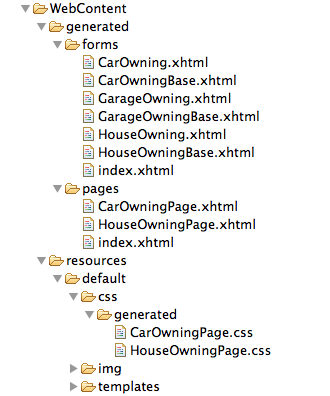
\includegraphics[width=10cm]{./images/chapter03/referenceimpl_projecttree_qls.png}

The page \emph{HouseOwningPage} contains two sections using the forms \emph{HouseOwning} 
and \emph{GarageOwning}, thus the generated file \emph{pages/HouseOwningPage.xhtml} composes
the two base files \emph{forms/HouseOwningBase.xhtml} and \emph{forms/GarageOwningBase.xhtml}
(generated by the QL code generator) together:

\begin{lstlisting}[language=HTML]
<html xmlns="http://www.w3.org/1999/xhtml"
      xmlns:ui="http://java.sun.com/jsf/facelets"
      xmlns:h="http://java.sun.com/jsf/html"
      xmlns:f="http://java.sun.com/jsf/core">
  <h:head></h:head>
  <ui:composition template="/index.xhtml">
    <ui:define name="content">
      <h:outputStylesheet library="default/css/generated" name="HouseOwningPage.css"  />
      <div><ui:include src="/generated/forms/HouseOwningBase.xhtml" /></div><p/>
      <div><ui:include src="/generated/forms/GarageOwningBase.xhtml" /></div>
  
  	  <div>
  	  <h:outputLink value="CarOwningPage.jsf">CarOwningPage</h:outputLink>
	  </div>
    </ui:define>
  </ui:composition>
</html>
\end{lstlisting}

The two pages are referenced in lines 9 and 10. Line 13 defines the link to the
next page as defined in the \texttt{navigation} section of the QLS model. Line 8
specifies which CSS file is to be used to render the site's elements. The CSS
file for the house owning page contains all corresponding styling information 
which are linked to the corresponding label elements by their ids:

\begin{lstlisting}[language=CSS]
#houseowning\:lblHasBoughtHouse {
	font-style:  italic; 	
}
#houseowning\:lblValueResidue {
	color:       #2233FF; 
	font-family: Verdana; 	
	font-weight: bold; 		
}
#garageowning\:lblHasBoughtGarage {
}
\end{lstlisting}

When JSF converts from Xhtml each element gets a unique (full qualified) id. In
out scenario this is always the id of the parent form concatenated with the id of
the elment itself. As separator JSF uses a colon. However, colons are special characters
in CSS, hence they need to be escaped.

Now that the intended artifacts to be generated are clearified, the code generator
itself can be written. Here again we use Xtend and some of its language concepts:

\begin{lstlisting}[language=Xtend]
class QlsDslGenerator implements IGenerator {
  @Inject extension JsfOutputConfigurationProvider
  @Inject extension JSFGenerator
  
  override void doGenerate(Resource input, IFileSystemAccess fsa) {
	if (input.URI.fileExtension!="qls")
      return
            
    val styleModel = input.contents.head as QuestionnaireStyleModel
    for (page: styleModel.pages) {
  	  val cssContent = generateCssFile(page);
   	  val cssFileName = "resources/default/css/generated/"+page.name+".css"
   	  fsa.generateFile(cssFileName, WEB_CONTENT, cssContent)
   	
   	  val xhtmlContent = generateXhtmlFile(page);
   	  val xhtmlFileName = "generated/pages/"+page.name+".xhtml"
   	  fsa.generateFile(xhtmlFileName, WEB_CONTENT, xhtmlContent)
    }
    val contentIndex  = generateIndexPage(styleModel.pages.get(0))
    fsa.generateFile("generated/pages/index.xhtml",WEB_CONTENT, contentIndex)
  }

  def generateCssFile(Page page) '''
  	<!-- @generated -->
    «FOR styleInfo: page.eAllContents.filter(typeof(StyleInformation)).toList»
		«styleInfo.id» {
		  «IF styleInfo.fontColor != null»color: «styleInfo.fontColor»;«ENDIF»
		  «IF styleInfo.fontFamily != null»font-family: «styleInfo.fontFamily»;«ENDIF»
		  «IF styleInfo.fontStyle != null»font-style: «styleInfo.fontStyle»;«ENDIF»
		  «IF styleInfo.fontWeight != null»font-weight: «styleInfo.fontWeight»;«ENDIF»
		}
   «ENDFOR»
  '''
	
  def generateXhtmlFile(Page page) '''
	<!-- @generated -->
	<html xmlns="http://www.w3.org/1999/xhtml"
	      xmlns:ui="http://java.sun.com/jsf/facelets"
	      xmlns:h="http://java.sun.com/jsf/html"
	      xmlns:f="http://java.sun.com/jsf/core">
	  <h:head></h:head>
	  <ui:composition template="/index.xhtml">
	    <ui:define name="content">
	      <h:outputStylesheet library="default/css/generated" name="«page.name».css"  />
	      «IF page.form != null»
	      <div><ui:include src="/generated/forms/«page.form.name»Base.xhtml" /></div>
	      «ELSE»
	        «FOR section: page.eAllContents.toList.filter(typeof(Section)).toList SEPARATOR '<p/>'»
	        <div><ui:include src="/generated/forms/«section.form.name»Base.xhtml" /></div>
	        «ENDFOR»
	      «ENDIF»
	  
	  	  <div>
	  	  «IF page.navigation != null»
	  	    «FOR nextPage: page.navigation.nextPage»
	  	    <h:outputLink value="«nextPage.name».jsf">«nextPage.name»</h:outputLink>
	  	    «ENDFOR»
	  	  «ENDIF»
		  </div>
	    </ui:define>
	  </ui:composition>
	</html>
  '''
    
  def generateIndexPage(Page page)'''
	<?xml version='1.0' encoding='UTF-8' ?>
	<!-- @generated -->
	<!DOCTYPE html PUBLIC "-//W3C//DTD XHTML 1.0 Transitional//EN" "http://www.w3.org/TR/xhtml1/DTD/xhtml1-transitional.dtd">
	<html xmlns="http://www.w3.org/1999/xhtml"
	      xmlns:h="http://java.sun.com/jsf/html"
	      xmlns:ui="http://java.sun.com/jsf/facelets">
	  <ui:composition template="/index.xhtml">
	    <ui:define name="content">
	      <h:outputLink value="«page.name».jsf">«page.name»</h:outputLink>
	    </ui:define>
	  </ui:composition>
	</html>
  '''	
	
  def getId(StyleInformation styleInfo) {
	val question = (styleInfo.eContainer as QuestionStyling).question
	val form = EcoreUtil2::getContainerOfType(question, typeof(Form))
	"#"+form.id+ "\\:lbl"+question.id.toFirstUpper
  }

  def dispatch getForm(Section section) {
	if (section.form != null) {
	  section.form
	}
	else {
	  section.eContainer.form
	}
  }
	
  def dispatch getForm(Page page) {
	page.form
  }
}

\end{lstlisting}




\section{Additional Concepts}

\subsection{Validation} \label{sec:validation}

As an optional task the LWC13 task requires the implementation of
analysis rules. Xtext provides a validation framework which integrates into the
EMF Validation
framework\footnote{\url{http://www.eclipse.org/modeling/emf/?project=validation}}.
The Xtext User Manual contains a Validation chapter that is
worth reading additionally\footnote{see
\url{http://www.eclipse.org/Xtext/documentation.html\#validation}}.

We will show in this section how the constraints defined in the task description
can be realized with Xtext.

\subsubsection{Extending the Java Validator class}
With the first translation of the Xtext grammar, the generator has already
created the necessary infrastructure to implement custom validation rules.
Look into the package \newline\texttt{org.eclipse.xtext.example.ql.validation},
you will find a Java class \texttt{QlDslJavaValidator}. The class extends the
\texttt{AbstractQlDslJavaValidator} class, which is regenerated each time the
grammar is translated. Thus, the generation gap pattern is applied here again.
It is safe to extend the \texttt{QlDslJavaValidator} class manually.

But instead of implementing the constraints in Java, we will use Xtend again.
For easier integration, our Xtend based validator class will be inserted into
the class hierarchy of \newline\texttt{QlDslJavaValidator}.

Create an Xtend class \texttt{QlDslXtendValidator}, and extend it from
\texttt{AbstractQlDslJavaValidator}.

\begin{lstlisting}[language=Xtend]
package org.eclipse.xtext.example.ql.validation

import javax.inject.Inject
import org.eclipse.xtext.validation.Check
import org.eclipse.xtext.xbase.XFeatureCall
import org.eclipse.xtext.xbase.XbasePackage
import org.eclipse.xtext.xbase.jvmmodel.IJvmModelAssociations

import static extension org.eclipse.xtext.nodemodel.util.NodeModelUtils.*
class QlDslXtendValidator extends AbstractQlDslJavaValidator {
  @Inject extension IJvmModelAssociations
}
\end{lstlisting}

Derive QlDslJavaValidator from the the Xtend validator:

\begin{lstlisting}[language=Java]
public class QlDslJavaValidator extends QlDslXtendValidator {
  // do nothing here, rules are implemented in Xtend
}
\end{lstlisting}

\subsubsection{Constraint: Ensure order of questions}

The first constraint in the LWC13 task is defined so:

\begin{quote}
\emph{
Test for cyclic dependencies. For instance, the following snippet should be rejected:
}
\begin{lstlisting}[language=QL]
if (x) { y: "Y?" boolean }
if (y) { x: "X?" boolean }
\end{lstlisting}

\emph{The reason is that y will only be asked for when x is true, but x will only get a value when y is true. 
Of course such cyclic dependencies could occur transitively and nested in expressions. 
Another way of stating this check is: the ordering of questions should be
consistent with how the question variables are used in conditions and computed values. 
}
\end{quote}

The task allows two approaches to achieve the goal. We will choose the second
approach: Check that elements referred in expressions have been declared before
their usage.

Xtext does not enforce that elements are declared before they are used
somewhere. The referred names simply must be in the scope of the context, which
the current scope implementation already accomplishes. We could implement this
constraint also in the scope provider of the language by restricting the scope
to elements that have been declared before. However, we will implement this as a
semantic constraint in the validator class.

To implement the constraint we need to know the location in the model where a
Question element is declared and where it is called in an expression. Besides
the Abstract Syntax Tree Xtext maintains a second model, which represents the
document. This is the so-called \emph{Node Model}, and the class
\texttt{NodeModelUtils} provides some utility functions to navigate from an AST
element to the node model. Since Questions that are referred in expressions are
local to the Form, we can simply compare the offset in the document of the
declared Question and the feature call in an expression.

Xtext validation rules are implemented as methods which are annotated with
\texttt{@Check}. The method name does not matter. Check methods are expected to
have exactly one parameter, which is of the type of element that has to be
checked. The base class provides methods to create error messages. For the case
of this constraint, the necessary context object type is \texttt{XFeatureCall}. 

Now open the \texttt{QlDslXtendValidator} class again and add this
method\footnote{\url{https://gist.github.com/kthoms/5240455}}:

\begin{lstlisting}[language=Xtend]
  @Check
  def void check_featureDeclaredBeforeCall (XFeatureCall featureCall) {
    val featureSource = featureCall.feature.sourceElements.head
    val nodeFeature = if (featureSource != null) featureSource.node else featureCall.feature.node
    val nodeCall = featureCall.node
    if (nodeFeature != null) {
      if (nodeFeature.offset > nodeCall.offset) {
        error(featureCall.feature.simpleName+" must be declared before.",featureCall, 
        XbasePackage::eINSTANCE.XAbstractFeatureCall_Feature, "ERR_FEATURE_CALL_BEFORE_DECLARATION", null)
      }
    }
  }
\end{lstlisting}

After restarting the workbench the situation will be recognized as an error:

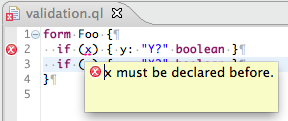
\includegraphics[width=6cm]{images/chapter04/validation_1.png}

\subsubsection{Constraint: Type conformance check}

Next, the LWC13 task requires checking the type conformance in expressions:

\begin{quote}
\emph{Type check conditions and variables: the expressions in conditions should be
type correct and should ultimately be booleans. The assigned variables should be
assigned consistently: each assignment should use the same type.
}\end{quote}

Here we have to do nothing, since this constraint is already implemented in
Xbase. This works thanks to Xbase's type inference mechanism. The Xtend language
makes heavy use of this nice feature, which makes it almost unneccessary to
declare types anywhere. For dynamic languages this is natural, since the actual
type is known and evaluated at runtime. Static typed language often lack this
feature.

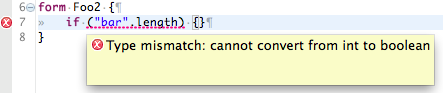
\includegraphics[width=6cm]{images/chapter04/validation_2.png}

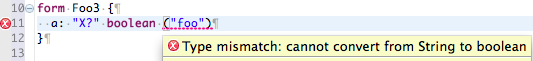
\includegraphics[width=6cm]{images/chapter04/validation_3.png}


\subsubsection{Testing validation rules}

It is easy to test validation rules in a runtime environment. However, we will
show how these rules can also be unit tested. Also herefore the Xtext framework
already contains the necessary infrastructure. Remember that Xtext has already
created a test plugin with the initial generator run? Now it is time to make use
of it.

Again, it is easier to create the test with Xtend. Xtend allows us to create
simple models inline with Rich Strings, pass the result to a parser, and
validate the result. With Xtend this is a one-liner.

\begin{lstlisting}[language=Xtend]
package org.eclipse.xtext.example.ql.validation.test

import javax.inject.Inject
import org.eclipse.xtext.example.ql.QlDslInjectorProvider
import org.eclipse.xtext.example.ql.qlDsl.Questionnaire
import org.eclipse.xtext.junit4.InjectWith
import org.eclipse.xtext.junit4.XtextRunner
import org.eclipse.xtext.junit4.util.ParseHelper
import org.eclipse.xtext.junit4.validation.ValidationTestHelper
import org.eclipse.xtext.xbase.XbasePackage
import org.junit.Before
import org.junit.Test
import org.junit.runner.RunWith

@RunWith(typeof(XtextRunner))
@InjectWith(typeof(QlDslInjectorProvider))
class QlDslValidationTest {
  @Inject extension ParseHelper<Questionnaire> parseHelper
  @Inject extension ValidationTestHelper
  
  @Before
  def void setUp () {
    parseHelper.fileExtension="ql"
  }
  
  @Test
  def void testValidation_CallBeforeDeclaration_expectError () {
    '''
    form Foo {
      if (x) { y: "Y?" boolean }
      if (y) { x: "X?" boolean }
    }
    '''.parse.assertError(XbasePackage::eINSTANCE.XFeatureCall, "ERR_FEATURE_CALL_BEFORE_DECLARATION", "must be declared before")
  }

  @Test
  def void testValidation_CallBeforeDeclaration_expectSuccess () {
    '''
    form Foo {
      x: "foo" boolean
      if (x) { a: "X?" boolean }
    }
    '''.parse.assertNoErrors
  }
  
  
  // Type check conditions and variables: the expressions in conditions should be type correct and should ultimately be booleans. 
  // The assigned variables should be assigned consistently: each assignment should use the same type.  
  @Test
  def void testValidation_ConditionTypeCheck_expectError () {
    '''
    form Foo {
      if ("foo".length) { a: "X?" boolean }
    }
    '''.parse.assertError(XbasePackage::eINSTANCE.XMemberFeatureCall, 
       "org.eclipse.xtext.xbase.validation.IssueCodes.incompatible_types", "Type mismatch")
  }
  
  @Test
  def void testValidation_ConditionTypeCheck_expectSuccess () {
    '''
    form Foo {
      if ("foo".length>1) { a: "X?" boolean }
    }
    '''.parse.assertNoErrors
  }

  @Test
  def void testValidation_AssignmentTypeCheck_expectFailure () {
    '''
    form Foo {
      a: "X?" boolean ("foo".length)
    }
    '''.parse.assertError(XbasePackage::eINSTANCE.XMemberFeatureCall, 
       "org.eclipse.xtext.xbase.validation.IssueCodes.incompatible_types", "Type mismatch")
  }

  @Test
  def void testValidation_AssignmentTypeCheck_expectSuccess () {
    '''
    form Foo {
      a: "X?" boolean ("foo".length>1)
    }
    '''.parse.assertNoErrors
  }
}
\end{lstlisting}

Basically, the class is a plain JUnit 4 class. We have to use a special
JUnit execution class, \texttt{XtextRunner}, and provide a language specific initializer
class, \texttt{QlDslInjectorProvider}.

Next, the class adds two extension classes. ParseHelper provides a parse()
method for char sequences. This will parse and validate the model. Afterwards
the observed issues can be asserted with the methods from the 

\begin{lstlisting}[language=Xtend]
@RunWith(typeof(XtextRunner))
@InjectWith(typeof(QlDslInjectorProvider))
class QlDslValidationTest { 
  @Inject extension ParseHelper<Questionnaire> parseHelper
  @Inject extension ValidationTestHelper
  ...
}
\end{lstlisting}

Now the test methods can be implemented. They are super simple:

\begin{lstlisting}[language=Xtend]
  @Test
  def void testValidation_CallBeforeDeclaration_expectSuccess () {
    '''
    form Foo {
      x: "foo" boolean
      if (x) { a: "X?" boolean }
    }
    '''.parse.assertNoErrors
  }
\end{lstlisting}
  
Due to the tight Java integration, the unit tests of the Xtend class can be
executed by running them through the context menu (\emph{Run As / JUnit Test}).

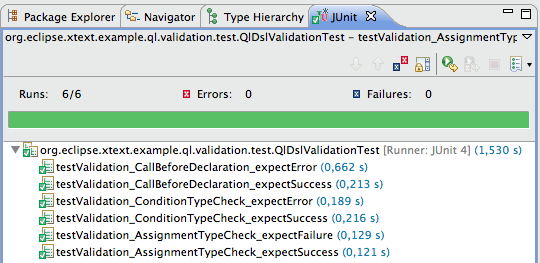
\includegraphics[width=12cm]{images/chapter04/validation_4.png}




\end{document}